\documentclass[12pt,english]{article}

\usepackage{amsmath,amssymb,amsthm,epsfig,lineno,rotfloat,psfrag,natbib,caption,setspace,url,bm,geometry}
\usepackage{ecology}

\geometry{verbose,letterpaper,tmargin=2.54cm,bmargin=2.54cm,lmargin=2.54cm,rmargin=2.54cm}

%\setlength{\evensidemargin}{0in} \setlength{\oddsidemargin}{0in}
%\setlength{\topmargin}{-0.65in} \setlength{\textwidth}{6.5in}
%\setlength{\textheight}{9.5in} \setlength{\topskip}{0in}
%\setlength{\headheight}{0in}

\bibpunct{(}{)}{,}{a}{}{;}

%\renewcommand{\includegraphics}[2][]{}

\bibliographystyle{ecology}
\raggedbottom


\captionsetup[table]{margin=0pt,font=small,labelfont={sc},justification=justified,labelsep=period}
\captionsetup[figure]{margin=0pt,font=small,labelfont={sc},justification=justified,labelsep=period,name=Fig}



\begin{document}
\begin{spacing}{1.9}


\begin{center}
A guide to Bayesian model checking for ecologists
\bigskip\\
\normalsize
{\sc Paul B. Conn$^{1,}$\footnotemark[5], Mevin B. Hooten$^{2,3,4}$,
Devin S. Johnson$^1$, and Peter L. Boveng$^1$}\smallskip\\
$^1${\em National Marine Mammal Laboratory, NOAA, National Marine Fisheries Service,
Alaska Fisheries Science Center, 7600 Sand Point Way NE, Seattle,
WA 98115 USA }\\ \medskip
$^2${\em U.S. Geological Survey, Colorado Cooperative Fish and Wildlife Research Unit, Colorado State University, Fort Collins, CO 80523 USA }\\ \medskip
$^3${\em Department of Fish, Wildlife, and Conservation Biology, Colorado State University, Fort Collins, CO 80523 USA }\\ \medskip
$^4${\em Department of Statistics, Colorado State University, Fort Collins, CO 80523 USA }\\ \medskip
\end{center}
\footnotetext[5]{Email: paul.conn@noaa.gov}


\raggedright \setlength{\parindent}{0.3in}
%\renewcommand{\baselinestretch}{1.8}\normalsize
\clubpenalty=0

\linenumbers

{\em Abstract.\ }  Checking that models adequately represent data an essential component of applied statistical inference.  Ecologists increasingly use hierarchical, Bayesian statistical models in their research.  The appeal of this modeling paradigm is undeniable, as researchers can build and fit models that embody complex ecological processes while simultaneously controlling for potential biases arising from sampling artifacts. However, ecologists tend to be less focused on checking model assumptions and assessing potential lack-of-fit when applying Bayesian methods than when they apply frequentist methods such as maximum likelihood.  There are also multiple ways of assessing goodness-of-fit for Bayesian models, each of which has strengths and weaknesses.  For instance, in ecological applications, the ``Bayesian p-value" is probably the most widely used approach for assessing lack of fit. Such p-values are relatively easy to compute, but they are well known to be conservative, producing p-values biased towards 0.5.  Alternatively, lesser known approaches to model checking, such as prior predictive checks, probability integral transforms, and pivot discrepancy measures may produce more accurate characterizations of goodness-of-fit but are not as well known to ecologists.  In addition, a suite of visual and targeted diagnostics can be used to examine violations of different model assumptions and lack-of-fit at different levels of the modeling hierarchy, and to check for residual temporal or spatial autocorrelation.  In this review, we synthesize existing literature in order to guide ecologists to the many available options for Bayesian model checking.  We illustrate methods and procedures with several ecological case studies, including i) explaining variation in spatio-temporal counts of bearded seals in the eastern Bering Sea, (ii) modeling the distribution of a herbaceous plant in in the Ozark Highlands of Missouri (USA), and (iii) using resource selection functions to model habitat preferences of XXX.  We argue that model checking is an essential component of scientific discovery and learning that should accompany Bayesian analyses whenever they are used to analyze ecological datasets.


{\em Bayesian p-value, Bayesian qq-plot, count data, goodness-of-fit diagnostic check, hierarchical model, model checking, occupancy, resource selection, pivot discrepancy, predictive distribution, probability interval transform, resource selection, spatio-temporal model}



\def\VAR{{\rm Var}\,}
\def\COV{{\rm Cov}\,}
\def\Prob{{\rm P}\,}
\def\bfX{{\bf X}\,}
\def\bfY{{\bf Y}\,}
\def\bfZ{{\bf Z}\,}
\def\bftheta{\boldsymbol{\theta}\,}
\def\bfeta{\boldsymbol{\eta}\,}


\section{Introduction}

Ecologists increasingly use Bayesian methods to analyze complex hierarchical models for natural systems \citep{HootenHobbs2015}.  Adoption of a Bayesian perspective requires that one specify prior distributions for model parameters, a process some have criticized for introducing unneeded subjectivity into the scientific process \citep{LeleDennis2009}.  However, there is a clear upside of making this Bayesian bargain: one can entertain models that were previously intractable using common modes of frequentist statistical inference (e.g., maximum likelihood). Ecologists are using Bayesian modes of inference to fit richer classes of models to their datasets, allowing them to model features such as temporal or spatial autocorrelation, individual level random effects, hidden states, and to separate the effects of process and measurement error \citep{LinkEtAl2002,ClarkBjornstad2004,CressieEtAl2009}.

Ultimately, the reliability of inferences from a fitted model (Bayesian or otherwise) are dependent on how well the model approximates reality.  There are multiple ways of assessing a model's performance in representing the system being studied. A first step is often to examine diagnostics that compare observed data to model output to pinpoint if and where any systematic differences occur. This process, which we term \textit{model checking}, is an integral part of statistical inference, as it helps diagnose assumption violations and illuminate places where a model might be amended to more faithfully represent gathered data. Following this step, one might proceed to compare the performance of alternative models embodying different hypotheses using any number of model comparison or out-of-sample predictive performance metrics \citep[see][for a review]{HootenHobbs2015} in order to gauge the support for alternative hypotheses or optimize predictive ability.  Note that scientific inference can still proceed if models do not fit the data well, but conclusions need to be tempered; one approach in such situations is to compute a variance inflation factor to adjust precision levels downward \citep[e.g.][]{BurnhamAnderson2002}.

Non-Bayesian statistical software often include a suite of goodness-of-fit diagnostics that allow practitioners to assess how well different models fit their data.  For instance, when fitting generalized linear \citep{McCullaghNelder1989} or additive \citep{Wood2006} models in the R programming environment \citep{RTeam2013}, one can easily access diagnostics such as quantile-quantile, residual, and leverage plots.  These diagnostics allow one to assess the reasonability of the assumed probability model, to examine whether there is evidence of heteroskedasticity, and to pinpoint outliers.  Likewise, in capture-recapture analysis there are established procedures for assessing overall fit as well as departures from specific model assumptions which are codified in user-friendly software such as U-CARE \citep{ChoquetEtAl2009}.  Results of such goodness-of-fit tests are routinely reported when publishing analyses in the ecological literature.

Somehow, the implicit requirement that one conduct model checking exercises does seems not to apply when reporting results of Bayesian analyses in the ecological literature.  For instance, a search of recent volumes of Ecology indicated that only 25\% of articles employing Bayesian analysis on real datasets reported any model checking or goodness-of-fit testing (Fig. 1).  We can think of several reasons why this might be the case.  First, it likely has to do with momentum; the lack of precedent in ecological literature may lead some authors looking for templates on how to publish Bayesian analyses to conclude that model checking is unnecessary.  Second, when researchers seek to publish new statistical methods, applications may be presented more as proof-of-concept exhibits than as definitive analyses that can stand up to scrutiny on their own. In such studies \citep[and textbooks; see e.g.,][]{RoyleDorazio2008}, topics like goodness-of-fit and model checking are often reserved for future research, presumably in journals with smaller impact factors.  We (the authors) are certainly guilty of presenting our research in this fashion.  Third, all of the articles we examined did a commendable job in reporting convergence diagnostics to support their contention that Markov chains from MCMC runs had reached their stationary distribution.  Perhaps there is a mistaken belief among authors and reviewers that convergence to a stationary distribution, combined with a lack of prior sensitivity, implies that a model fits the data?  Finally, it may just be that those publishing Bayesian analyses in ecological literature ``. . . like artists, have the bad habit of falling in love with their models" (to borrow a quote attributed to G.E.P. Box and referenced by \citet{LinkBarker2010} with regard to model checking).  We are certainly guilty of this fault as well.  Indeed this monograph can be viewed as a partial atonement for unrequited love.

If we accept the premise that Bayesian models in ecology should be routinely checked for compatibility with data, a logical next question is how best to conduct such checks.  Unfortunately, there is no single best answer.  Most texts in ecology \citep[e.g.][]{KingEtAl2009,LinkBarker2010,KerySchaub2012} focus on posterior predictive checks, as pioneered by \citet{Guttman1967}, Rubin (\citeyear{Rubin1981,Rubin1984}) and \citet{GelmanEtAl1996} (among others).  These procedures are also the main focus of the popular Bayesian analysis text by \citet{GelmanEtAl2004} and are based on the intuitive notion that data simulated from the posterior distribution should be similar to the data one is analyzing.  However, ``Bayesian p-values" generated from these tests tend to be conservative (biased towards 0.5) since the data are in effect used twice \citep[once to fit the model and once to test the model;][]{BayarriBerger2000,RobinsEtAl2000}.  By contrast, other approaches less familiar to ecologists (e.g. such as prior predictive checks, probability integral transforms, and pivot discrepancy measures) may produce more accurate characterizations of goodness-of-fit but may require extra data (for out-of-sample prediction), or may be more difficult to implement.

In this monograph, we seek to collate and digest relevant statistical literature with the goal of providing ecologists with a practical guide to Bayesian model checking.  We start by defining a consistent notation that we use throughout the paper. Next, we work to compile a bestiary of Bayesian model checking procedures, providing positives and negatives associated with each approach.  After describing several ways in which model checking results can sometimes be misleading (as with hierarchically centered models), we illustrate Bayesian model checking using three case studies.  These include a species distribution model (SDM) developed from bearded seal counts (\textit{Erignathus barbatus}) in the Chukchi Sea, an SDM developed from presence-absence data of a herbaceous plant (\textit{Genus species}) in Missouri, and analysis of animal telemetry data.  We conclude with several recommendations on how model checking results should be presented in the ecological literature.



\section{Background and notation}

\section{Model checking procedures}

\subsection{Posterior predictive checks (and the Bayesian p-value)}

algorithm description

example of p-values not being uniformly distributed

More power to detect differences if discrepancy measure does not depend on unknown parameters \citep[][Chapter 8]{LunEtAl2013}.  Plug in (i.e. $\hat{\theta}$

\subsection{Prior predictive checks}

\citet{Box1980} argued that the hypothetico-deductive process of scientific learning can be embodied through successive rounds of model formulation and testing. According to his view, models are built to represent current theory and an investigator's knowledge of the system under study; data are then collected to evaluate how well the existing theory (i.e., model) matches up with reality.  If necessary, the model under consideration can be amended, and the process repeats itself.  These Model checking is an integral part of the scientific enterprise in the modern era, including the study of ecology.  For instance,

From a Bayesian standpoint, such successive rounds of \textit{estimation} and \textit{criticism} are embodied through posterior inference and model checking, respectively \citep{Box1980}. 

If one views a model, complete with all its set of assumptions and prior beliefs

relationship to approximate Bayesian computation?

\subsection{Direct chi-square testing}

\citet{Johnson2004}

\subsection{Probability integral transforms}

\subsection{Pivoting discrepancy}

\citet{YuanJohnson2012}

\subsection{Just build a bigger model!  Tradeoffs between fit and prediction}

\section{Avoiding potential traps with model checking}

Mean structure vs. dispersion - not always obvious where misspecification occurs.

Hierarchical centering

\section{Examples}

\subsection{Modeling the distribution of a herbaceous plant}

\subsection{Spatio-temporal bearded seal counts}

\subsection{Resource selection of XXX}

\section{Discussion}


Focus on prior sensitivity, convergence diagnostics and sometimes model comparison (e.g. DIC or cross validation) - not as much focus on GOF.

GOF on most general model, then model selection/comparison/averaging \citep{BurnhamAnderson2004}.

path structure - directional/separation tests

\centerline{\sc Acknowledgments} Funding
for Bering Sea aerial surveys was provided by the U.S. National Oceanic and Atmospheric
Administration and by the U.S. Bureau of Ocean Energy Management (Interagency
Agreement M12PG00017).  The views and conclusions in this article represent the views of the authors and the U.S. Geological Survey but do not necessarily represent findings or policy of the U.S. National Oceanic and Atmospheric Administration.  Any use of trade, firm, or product names is for descriptive purposes only and does not imply endorsement by the U.S. Government.

\renewcommand{\refname}{Literature Cited}
\bibliography{master_bib}



\pagebreak

TABLES

\begin{table}[ht]
\caption{Example discrepancy functions for predictive checks.
}
\centering
\begin{tabular}{lcr}
  \hline
  Name & Definition & Comments \\
  \hline
  \multicolumn{3}{l}{\textbf{A. Omnibus discrepancy functions}} \\
  $\chi^2$ & $T(\textbf{y},\boldsymbol{\theta}) = \sum_i (y_i - E(y_i|\boldsymbol{\theta}))^2/\textrm{var}(y_i|\boldsymbol{\theta})$ & Often used for count data for count data; suggested by \citet{GelmanEtAl2004} (among others).\\
  Deviance ($D$) &  $T(\textbf{y},\boldsymbol{\theta}) = -2 \log [{\bf y} | \boldsymbol{\theta}]$ & \citep{KingEtAl}\\
  Likelihood ratio statistic & $T(\textbf{y},\boldsymbol{\theta}) = 2 \sum_i y_i \log(y_i/E(y_i|\boldsymbol{\theta}))$ & \citep{LunnEtAl2013} \\
  \multicolumn{3}{l}{\textbf{B. Targeted discrepancy functions}} \\
  Proportion of zeros & $T(\textbf{y}) = \sum_i I(y_i = 0) $ & Zero inflation check for count data \\
  Skewness checks & $T(\textbf{y}) = y_{p\%} $ & Using the $p\%$ quantile can be useful for checking for over- or underdispersion. \\
\hline
\end{tabular}
\end{table}

\pagebreak

FIGURE CAPTIONS

FIGURE 1.  Type of model checking procedures used in $n=31$ articles published in the journal Ecology during 2014 and 2015. Articles were found via a Web of Science for articles including the topic ``Bayesian" (search conducted 10/1/2015).  Six articles were determined to be non-applicable (N/A) because they either (1) were simulation studies, or (2) used approximate Bayesian computation, which is conceptually different than traditional Bayesian inference \citep[see e.g.][]{BeaumontEtAl2002}.  Of the remaining 25, 20 did not report any model checking procedures.  Five articles reported specific model checking procedures, which included a combination of Bayesian cross validation (\textit{Cross.val}, ), frequentist software (\textit{Non-Bayes}, posterior predictive p-values (\textit{Pp.pval}), and posterior predictive graphical checks (\textit{Pp.gc}).


\pagebreak

\begin{figure*}
\begin{center}
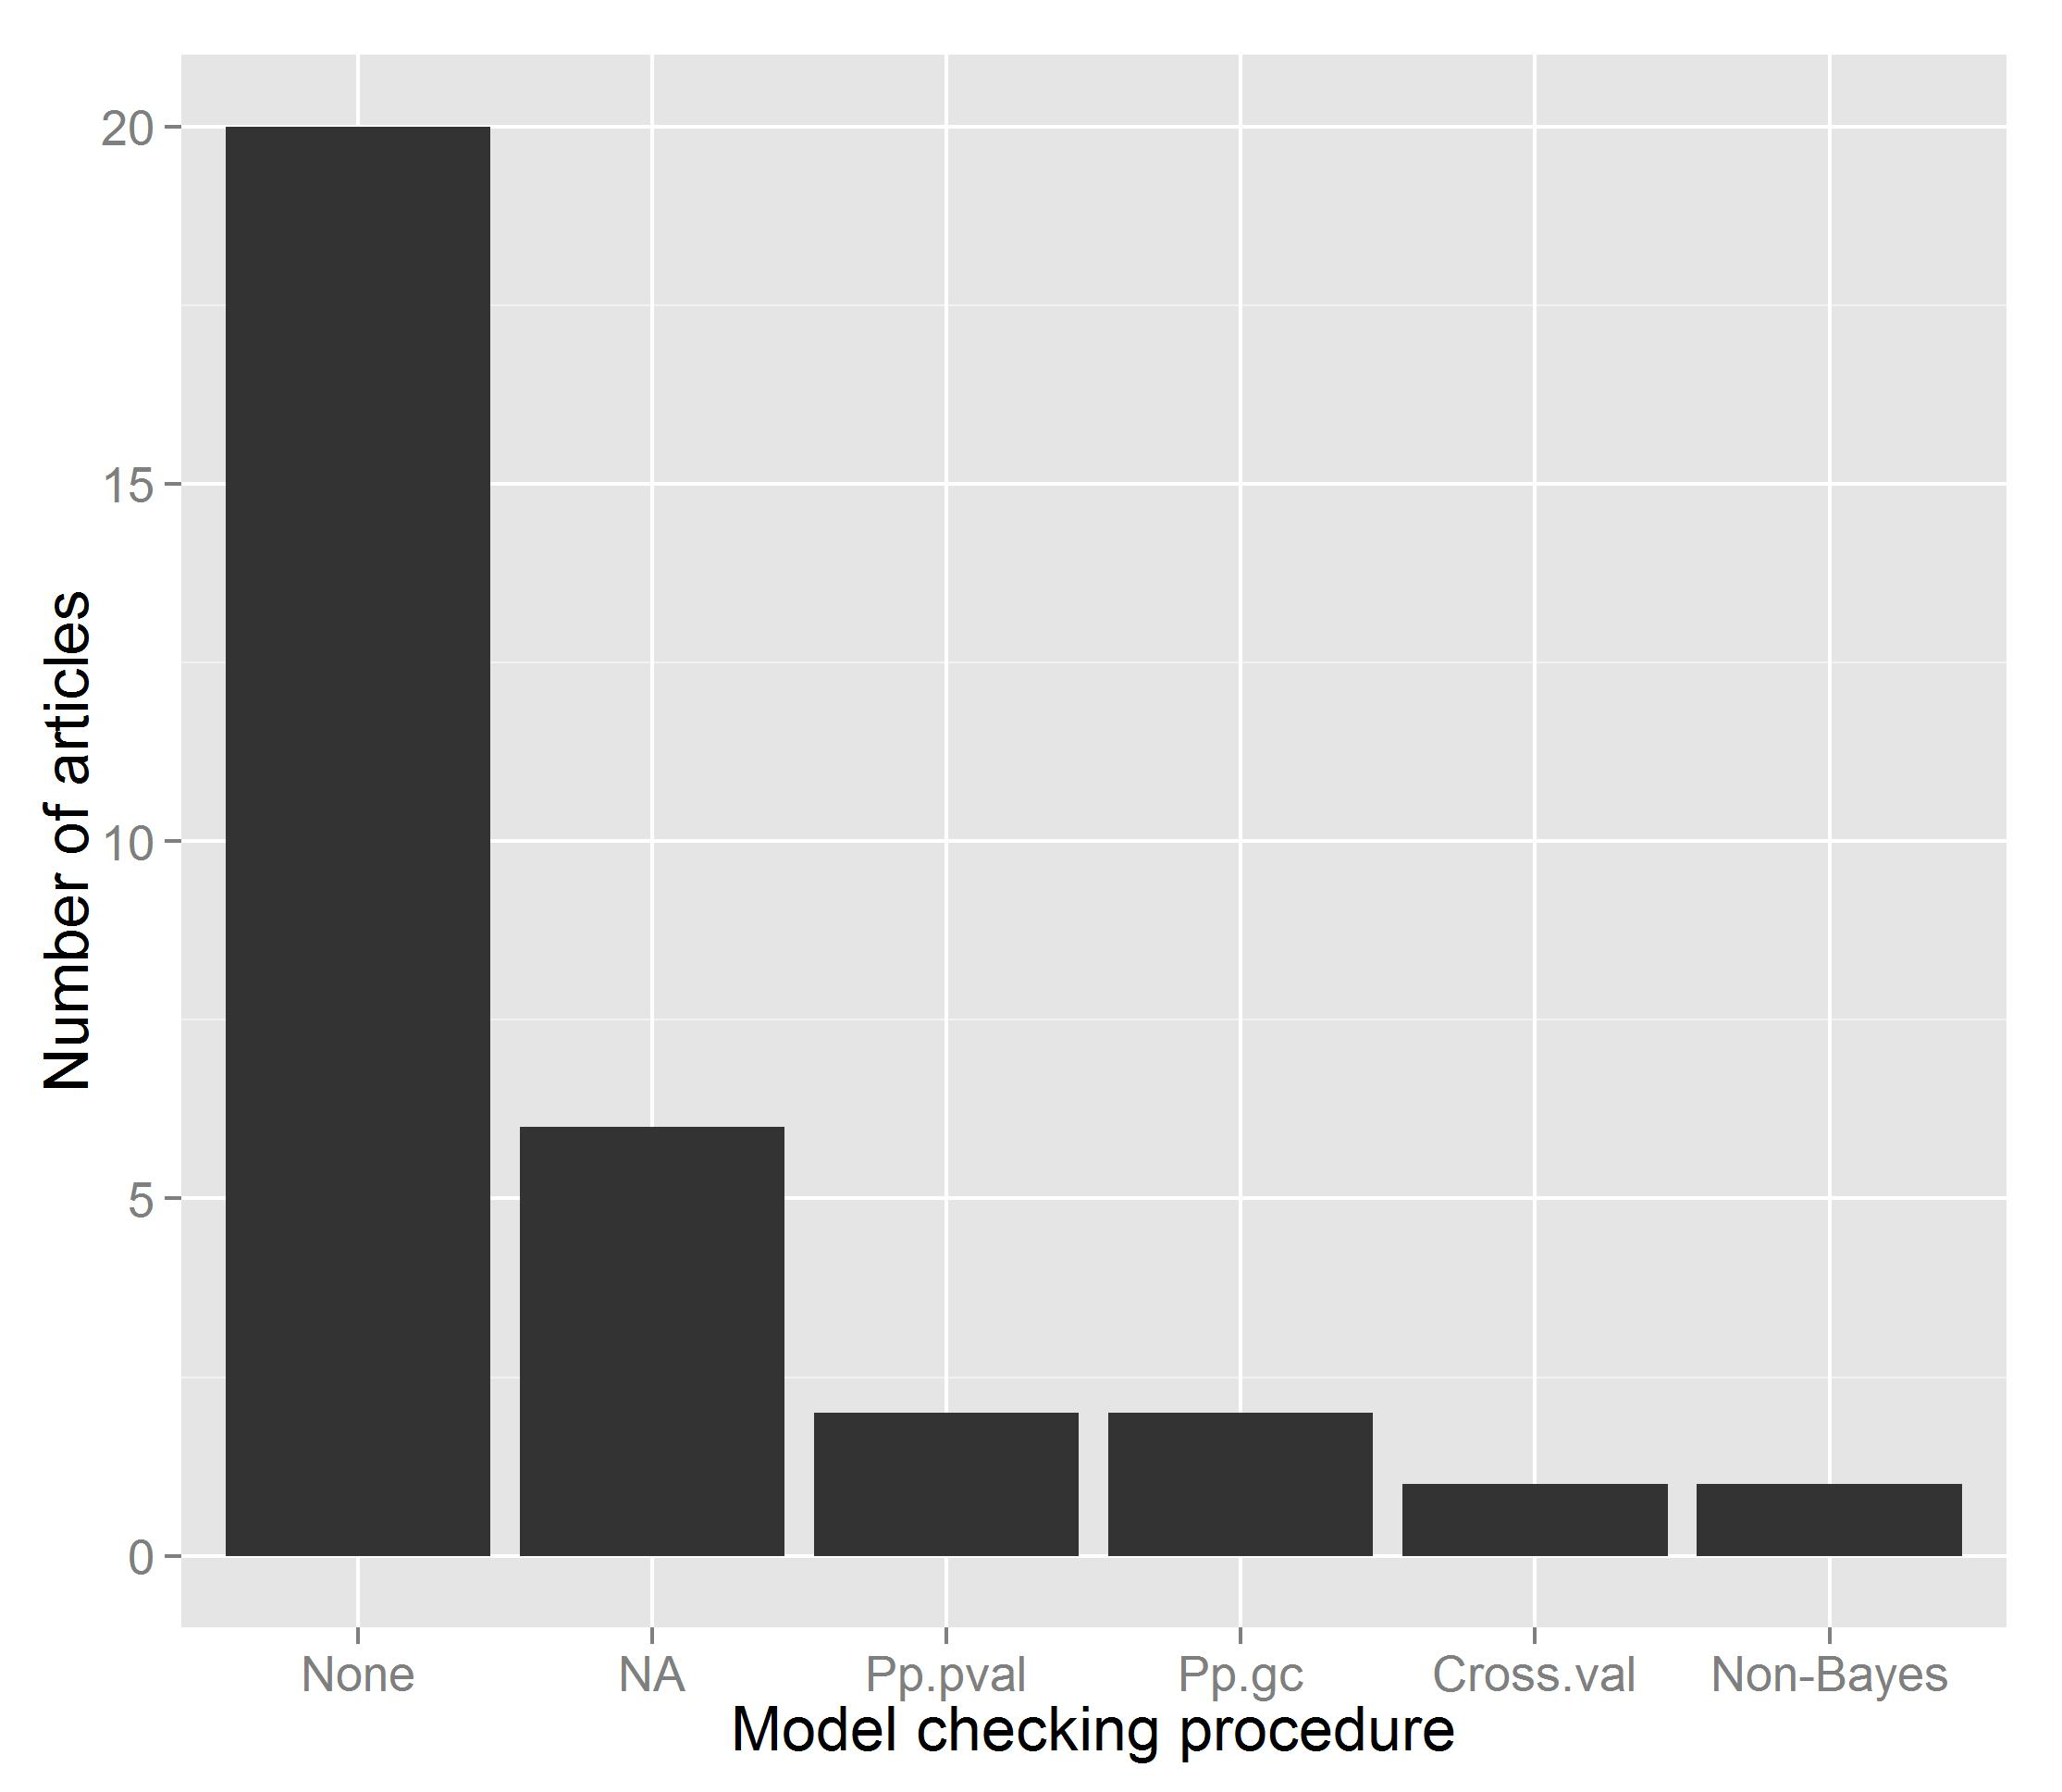
\includegraphics[width=170mm]{WOSsearch.jpeg}
\caption{} \label{fig:WOS}
\end{center}
\end{figure*}

\end{spacing}
\end{document}
